\chapter{Entwurf}
\label{ch:3}

\section{Klassendiagramm}
\label{sec:3.1}
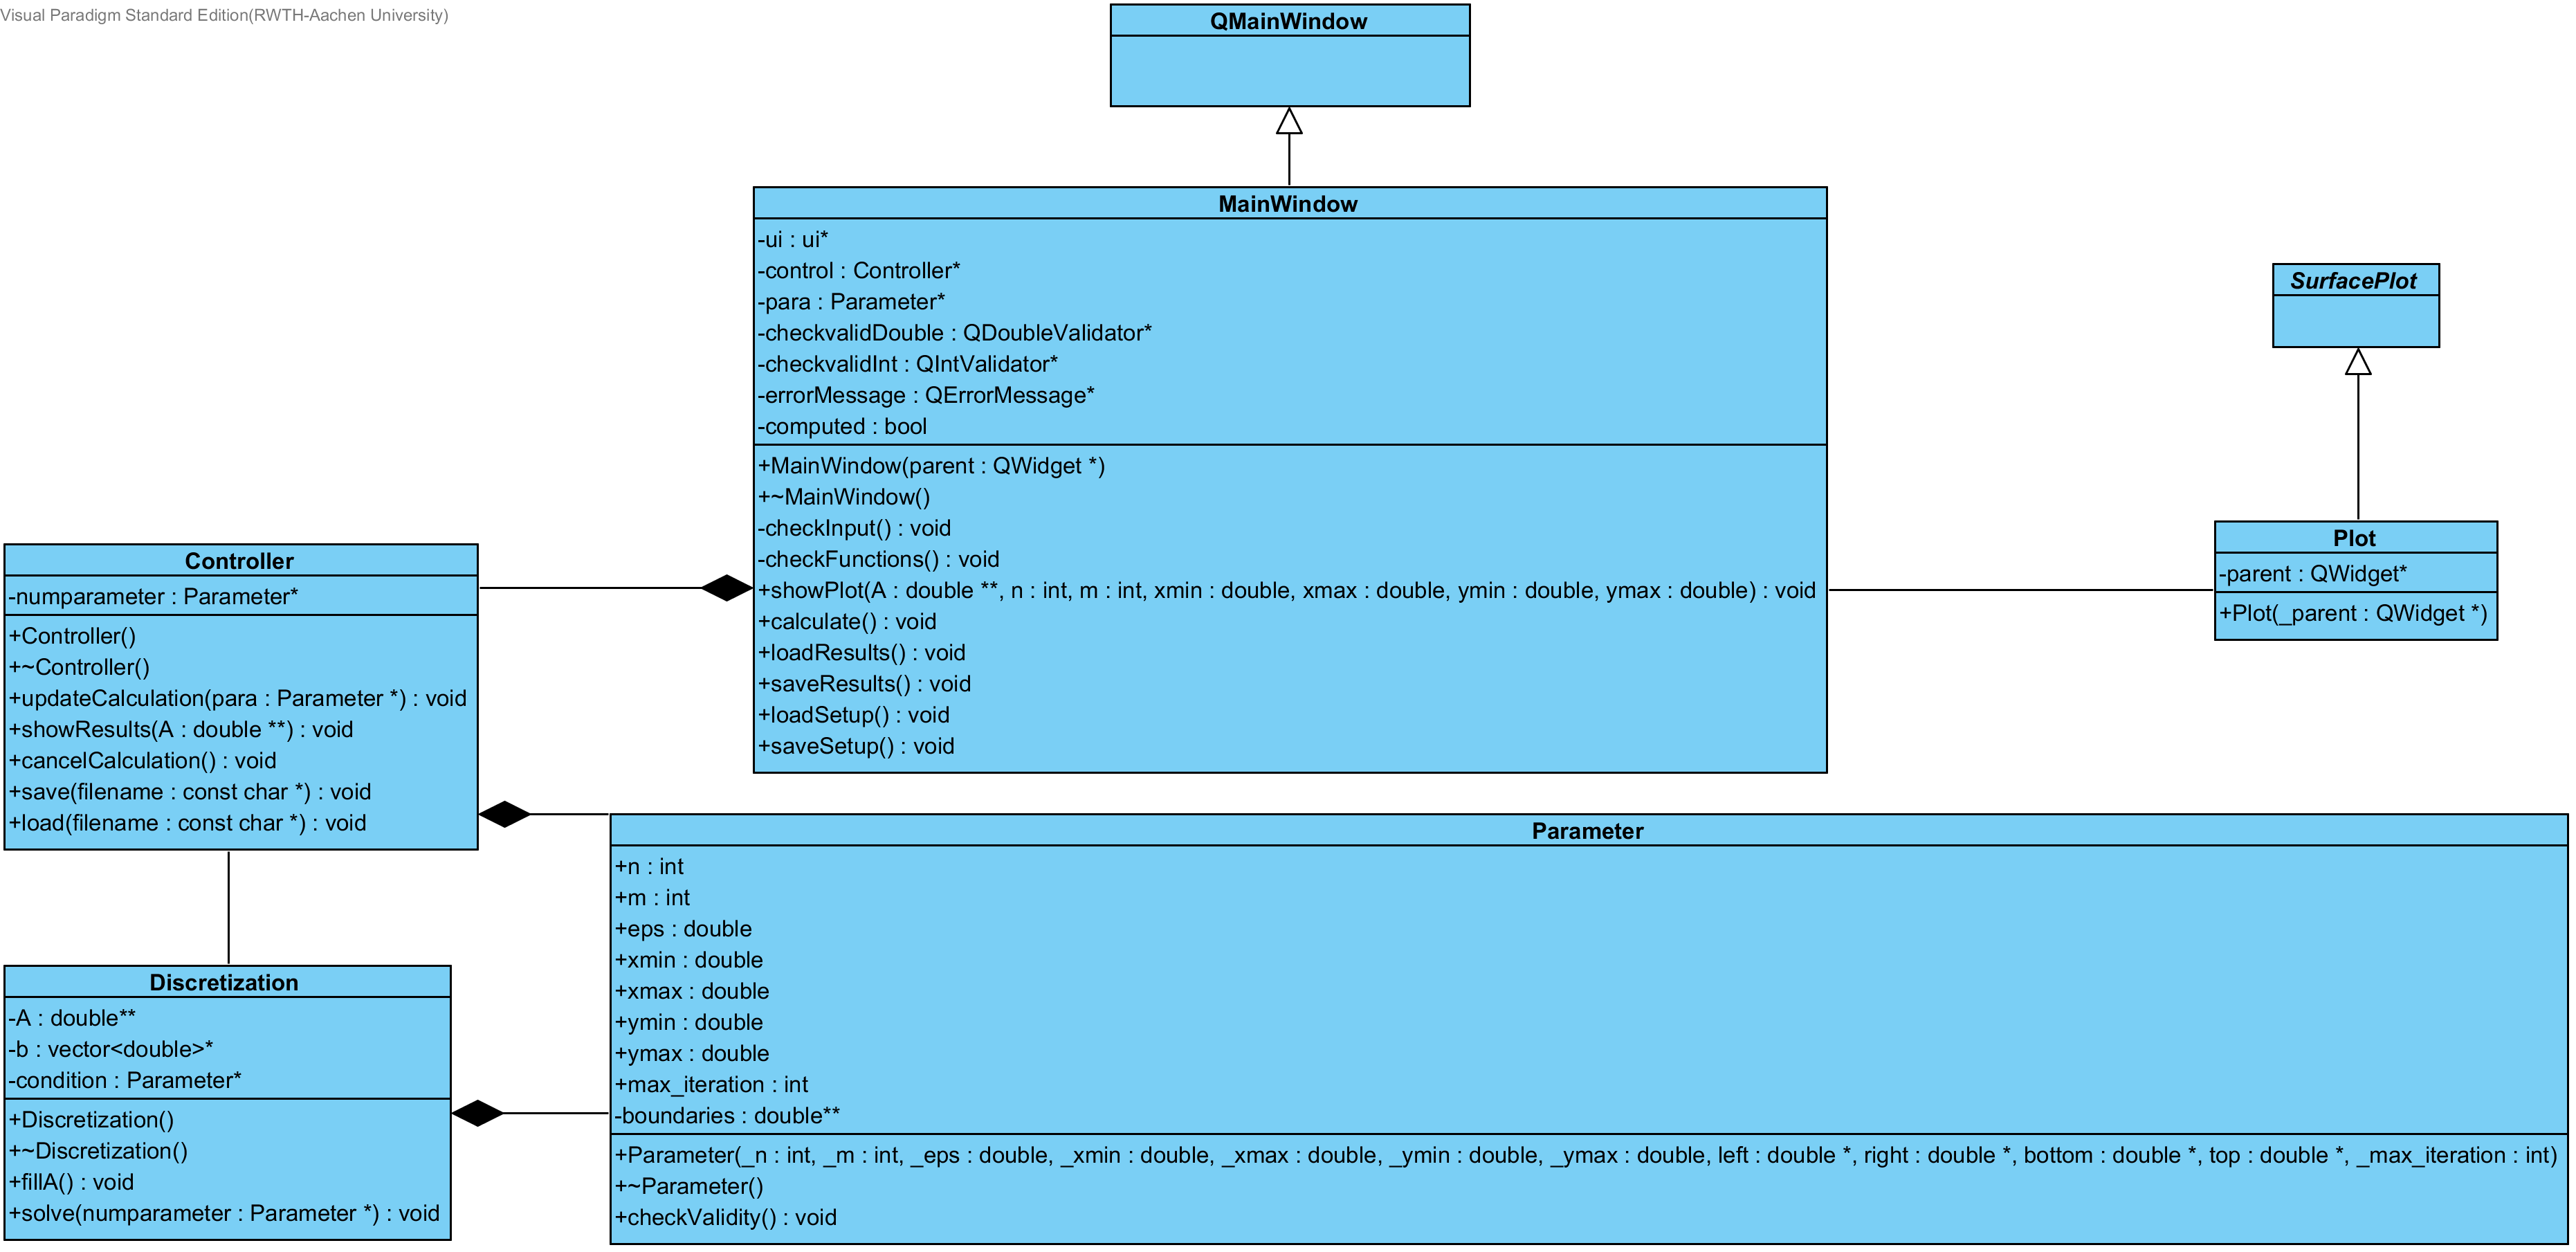
\epsfig{file=Bilder/Klassendiagramm.eps,width=\textwidth}

\section{Dynamik}
\label{sec:3.2}

\subsection{Sequenzdiagramme}

 \textbf{Beenden} \\ \newline 
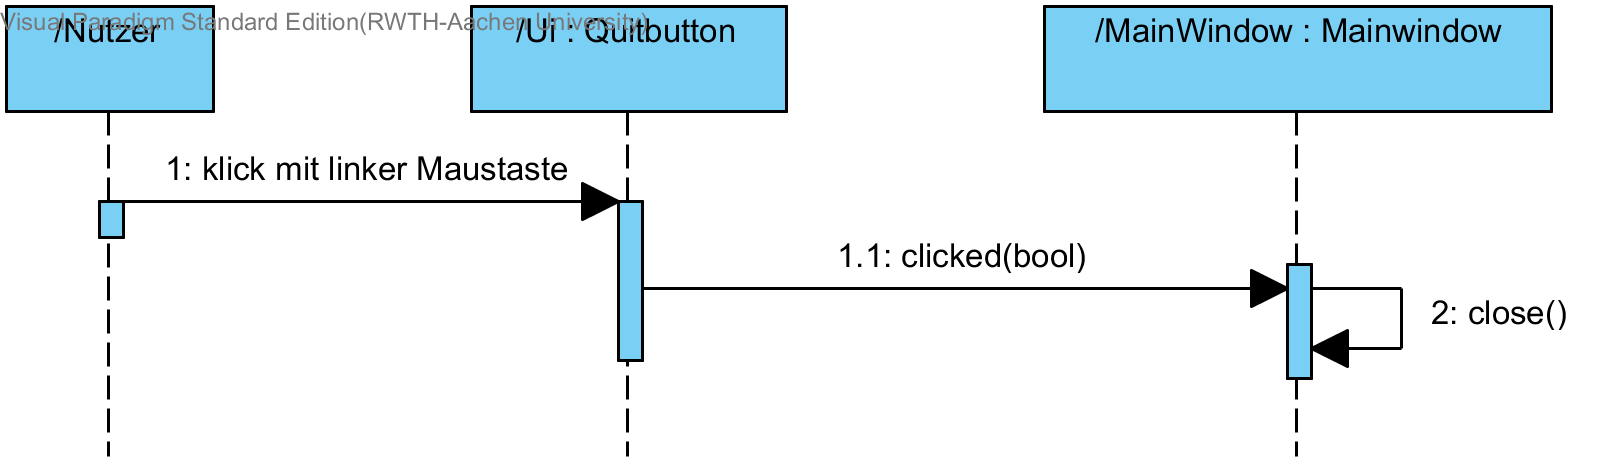
\epsfig{file=Bilder/Beenden.eps,width=\textwidth}
\newline \newline
 \textbf{Check Input} \\
\epsfig{file=Bilder/CheckInput.eps,width=\textwidth}
\newline \newline
 \textbf{Check Randfunktionen} \\
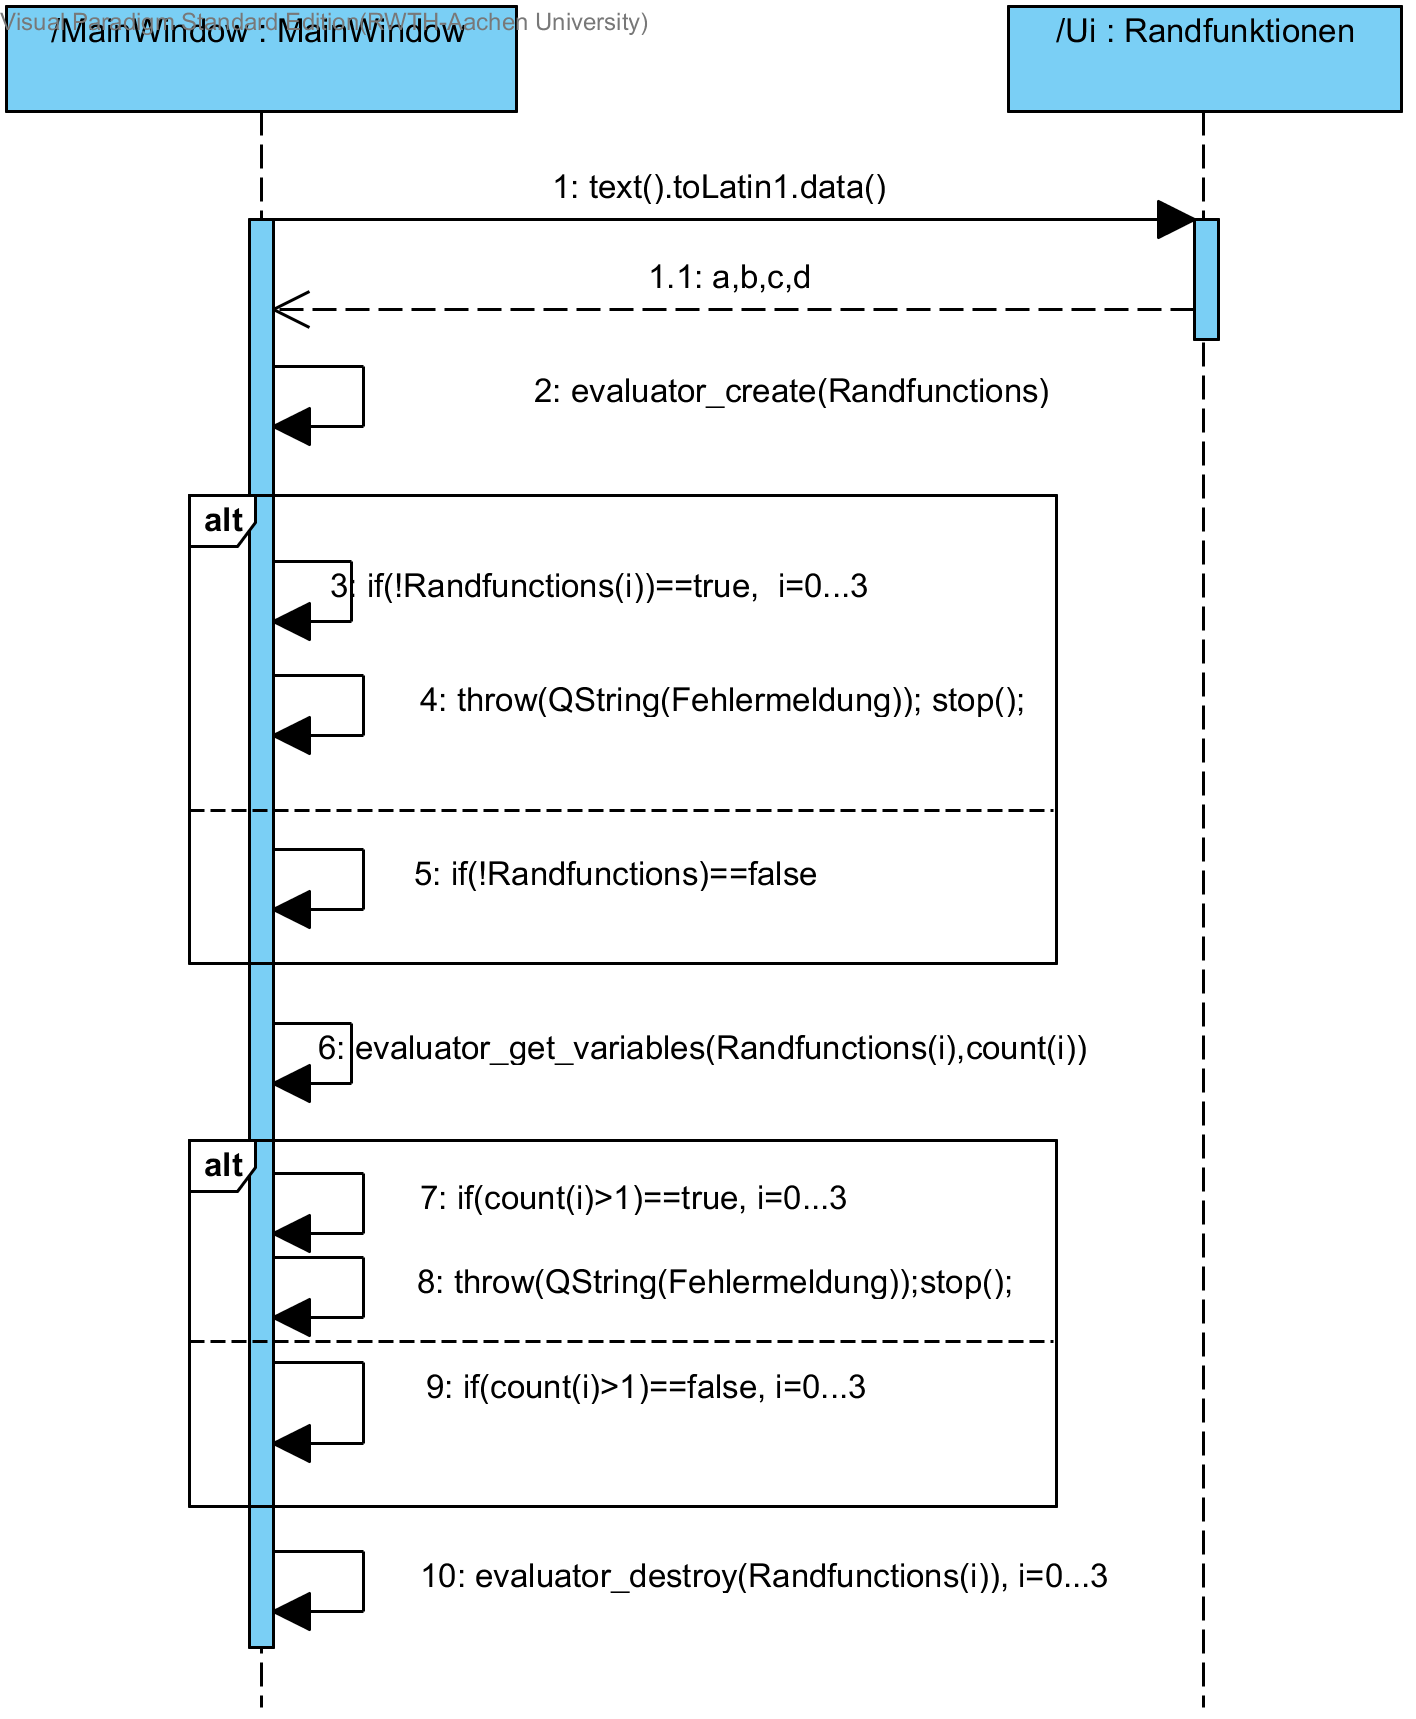
\epsfig{file=Bilder/checkRandfunktionen.eps,width=\textwidth}
\newline \newline
 \textbf{Einstellungen laden} \\
 \newline \newline
\epsfig{file=Bilder/Einstellungen_Laden_1.eps,width=\textwidth}
 \textbf{Einstellungen speichern} \\ \newline
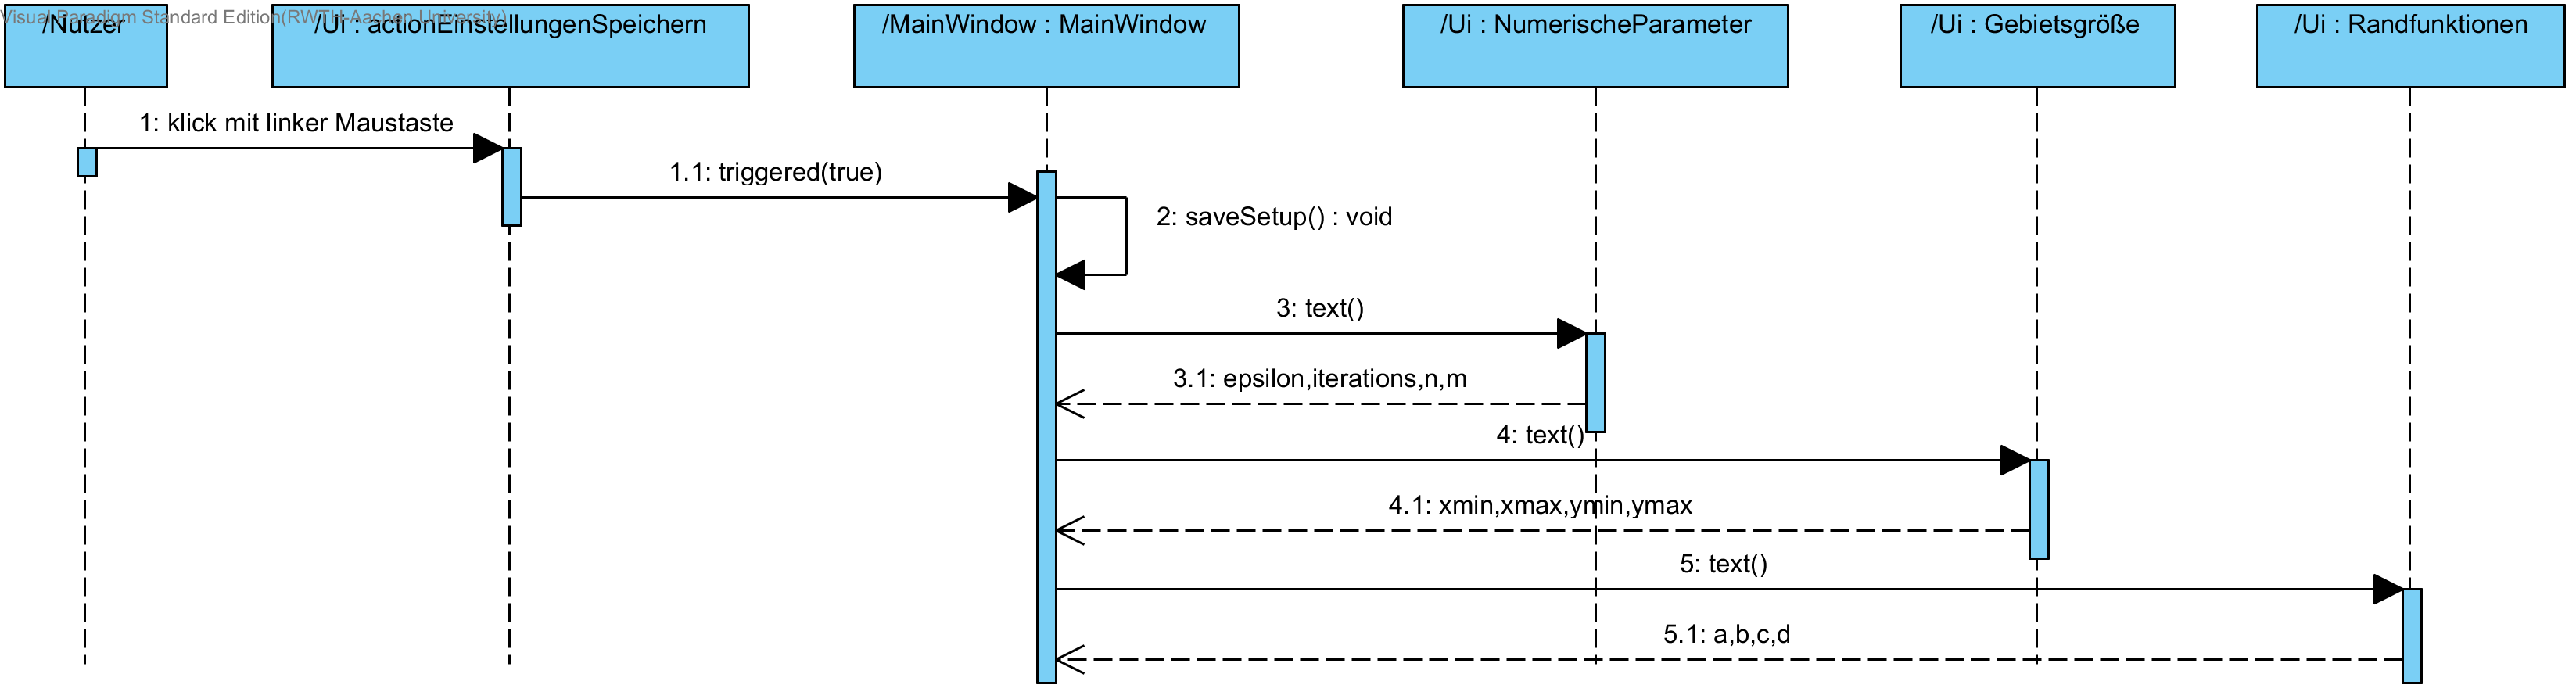
\epsfig{file=Bilder/Einstellungen_Speichern.eps,width=\textwidth}
 \textbf{Ergebnis laden} \\ \newline
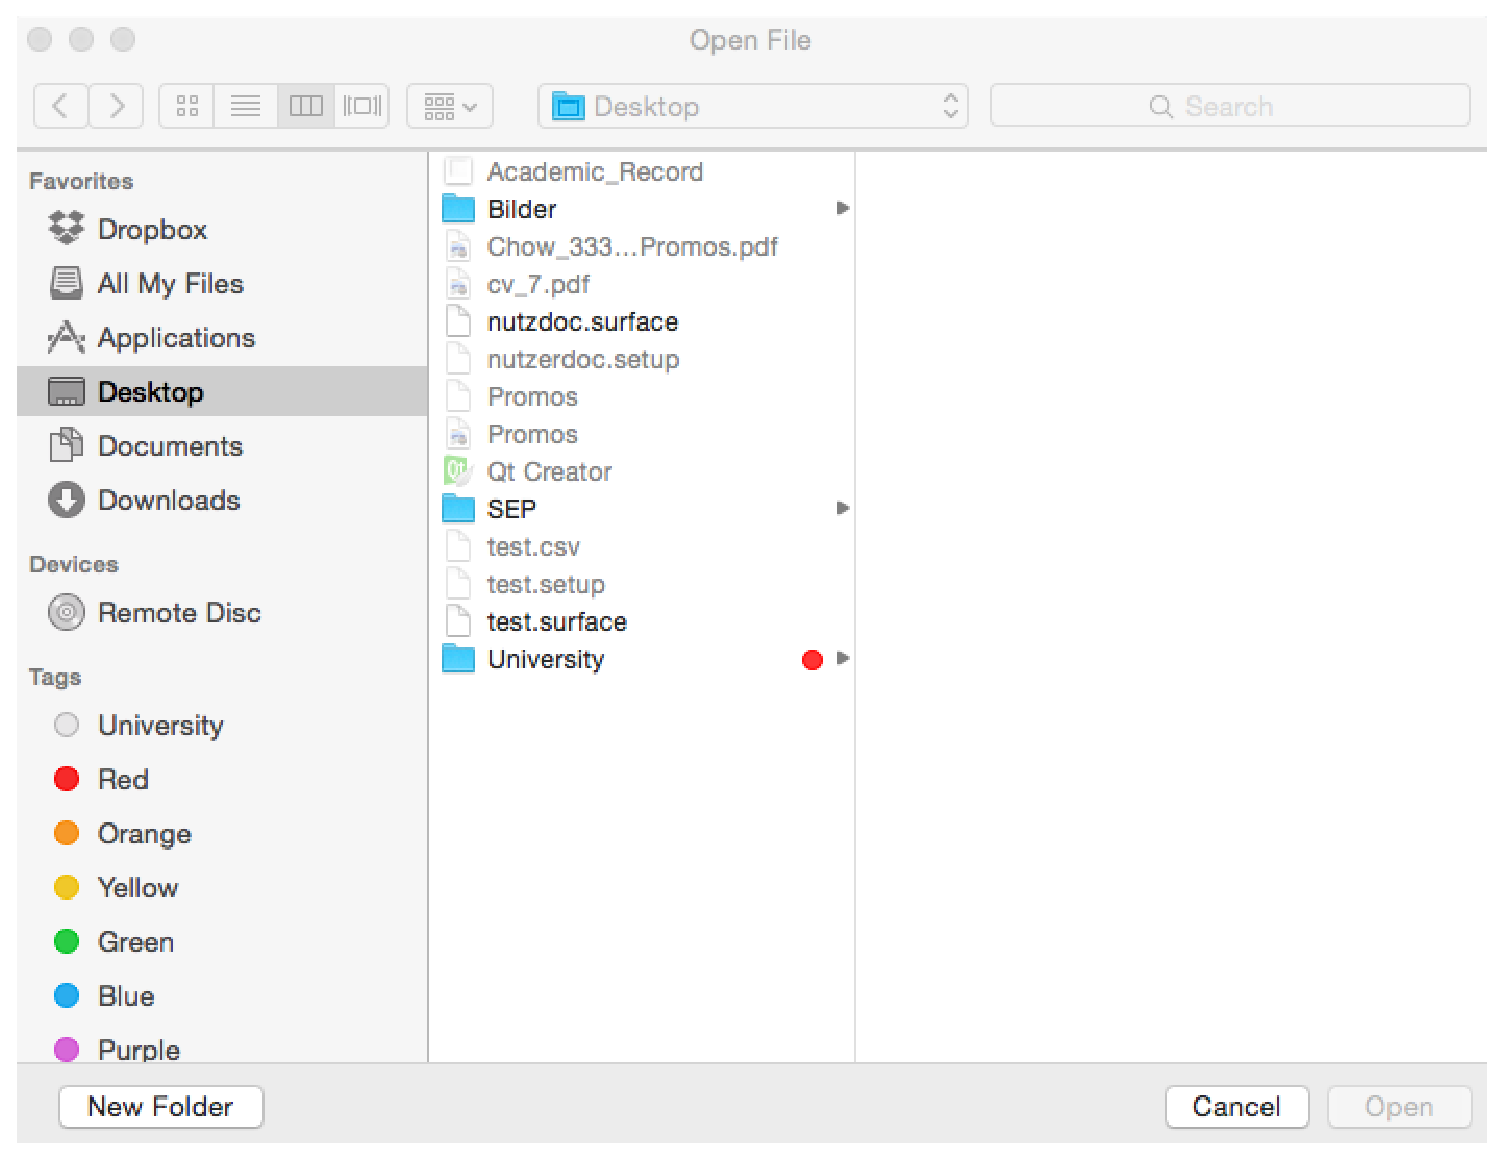
\epsfig{file=Bilder/Ergebnis_Laden.eps,width=\textwidth}
 \textbf{Ergebnis speichern} \\ \newline
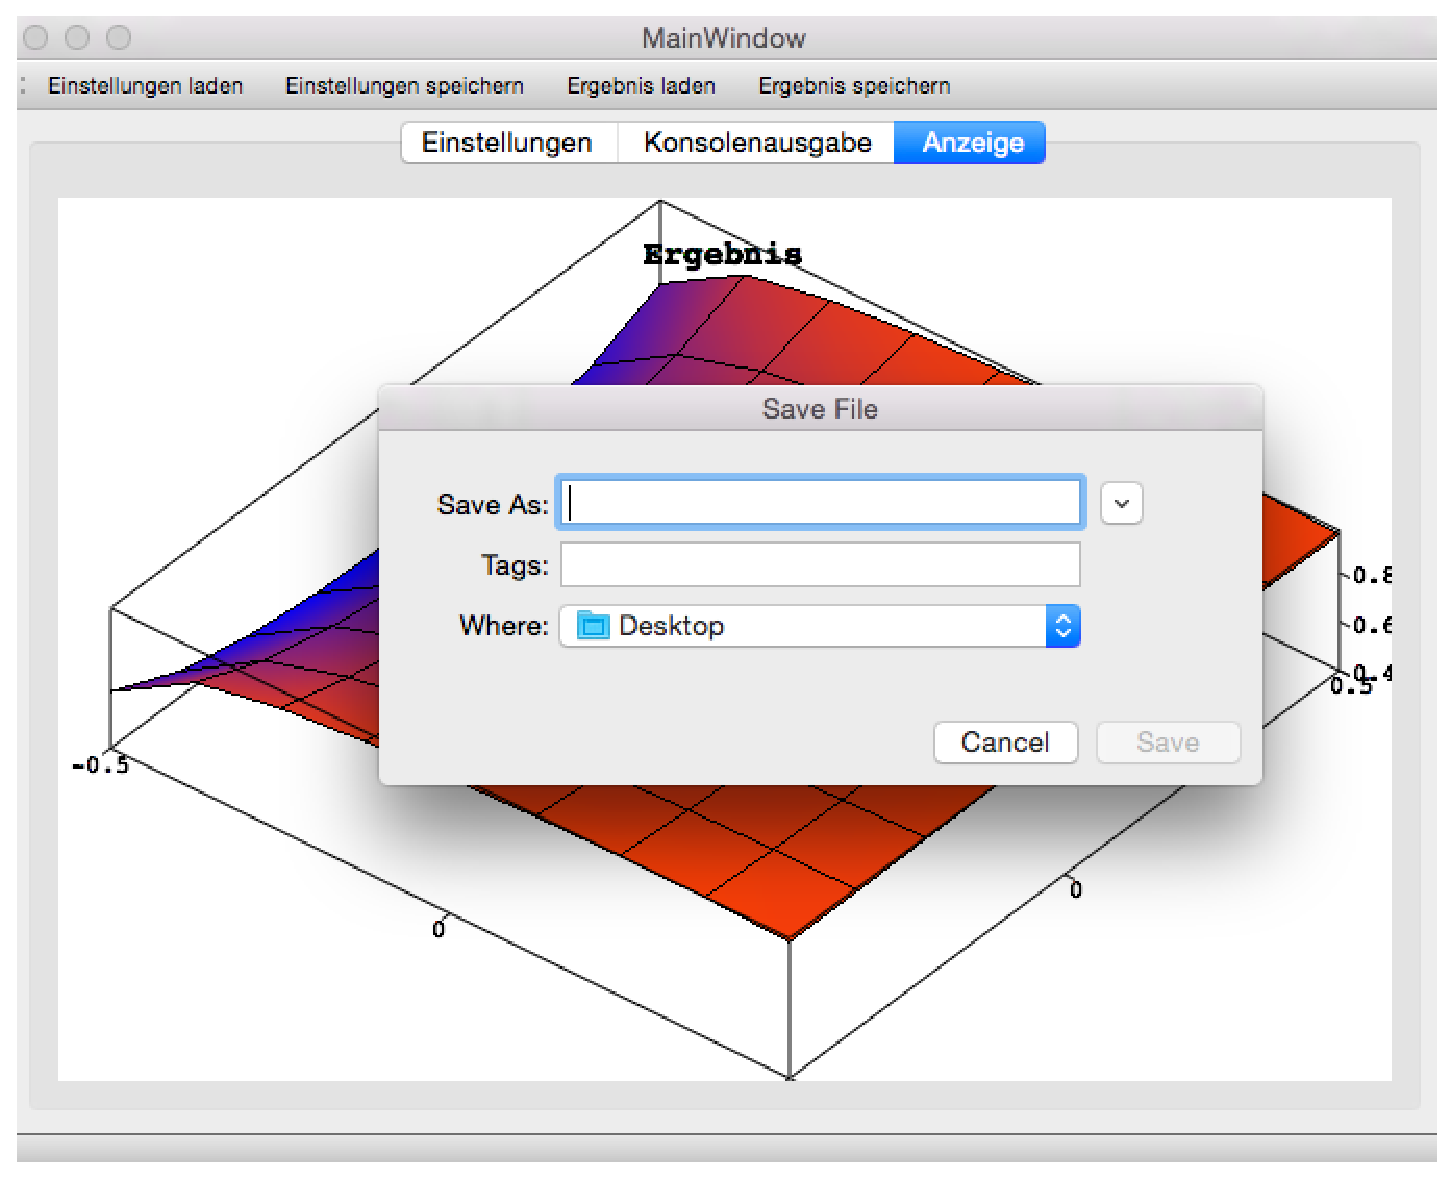
\epsfig{file=Bilder/Ergebnis_Speichern.eps,width=\textwidth}
 \textbf{Gebietsgr\"o\ss e \"andern} \\ \newline
\epsfig{file=Bilder/Gebietsgroesse_aendern.eps,width=\textwidth}
 \textbf{Numerische Parameter \"andern} \\ \newline
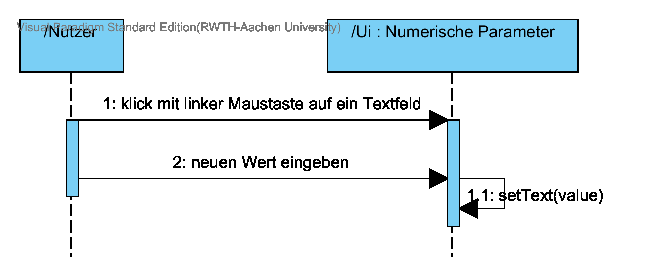
\epsfig{file=Bilder/NumerischeParameterAendern.eps,width=\textwidth}
 \textbf{Randfunktionen \"andern} \\ \newline
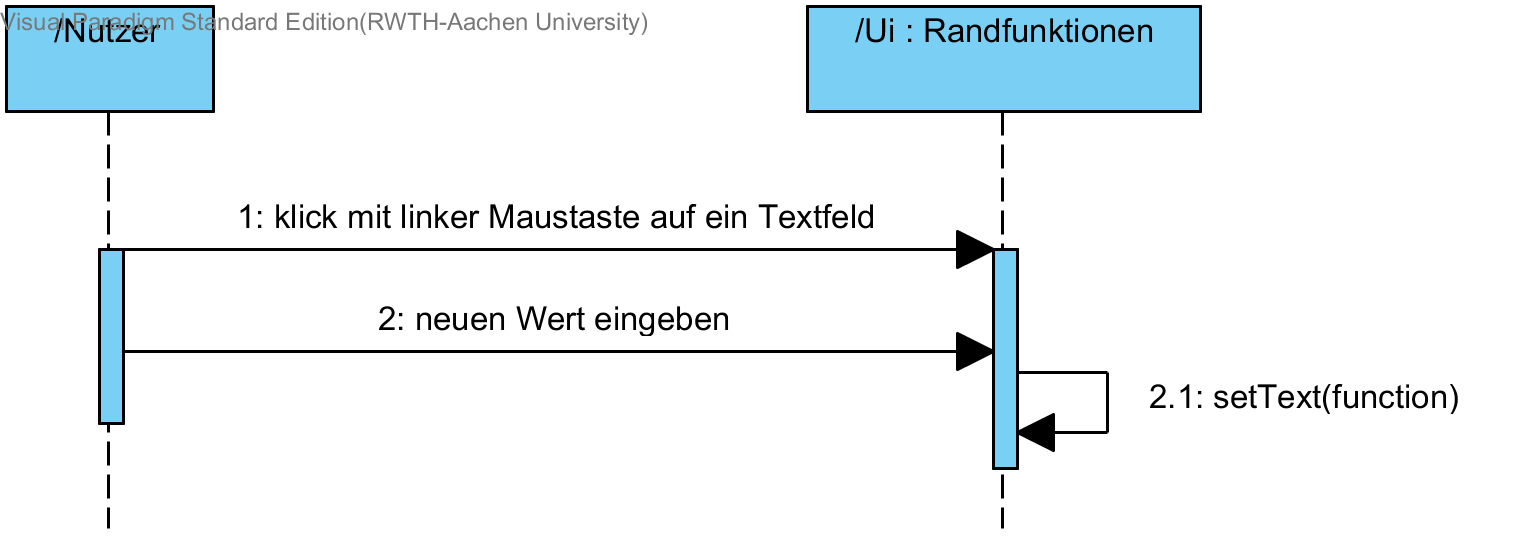
\epsfig{file=Bilder/RandfunktionenAendern.eps,width=\textwidth}
 \textbf{Run} \\ \newline
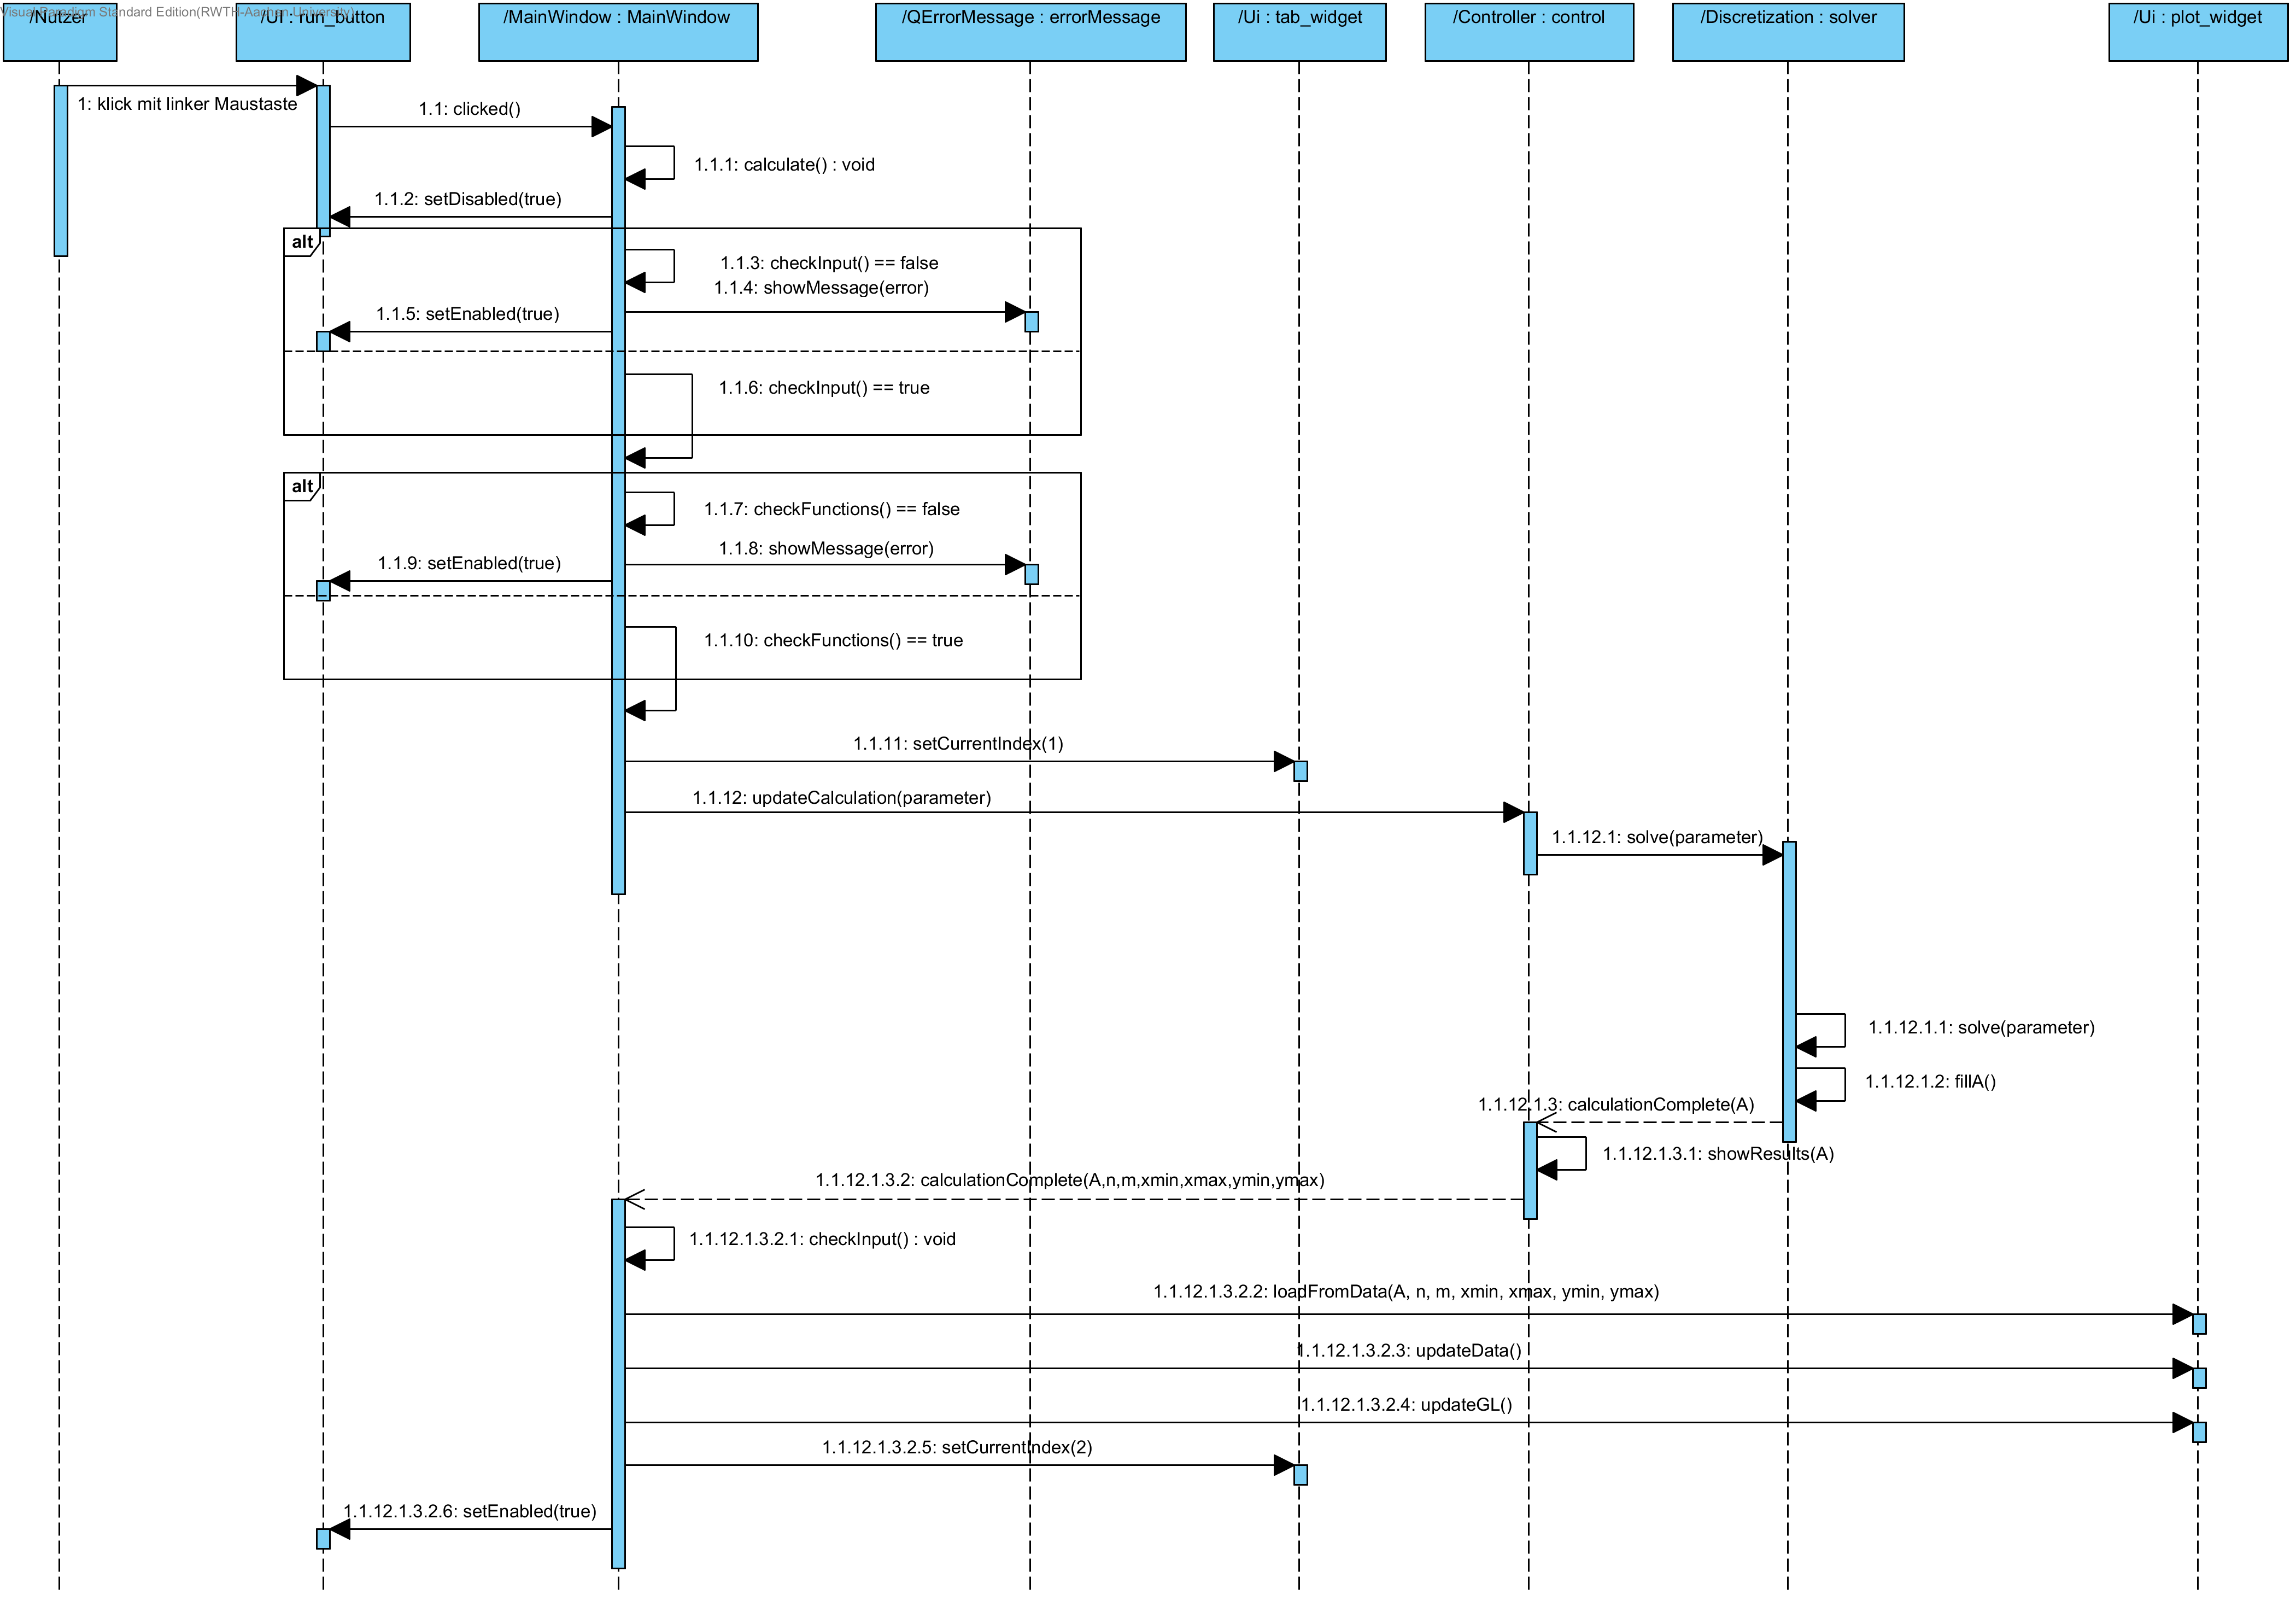
\epsfig{file=Bilder/Run.eps,width=\textwidth}
 \textbf{Tab wechseln} \\ \newline
\epsfig{file=Bilder/Tab_wechseln.eps,width=\textwidth}